\subsection{Rot-Schwarz-Baum}\label{s:rb_tree}
Der Rot-Schwarz-Baum stellt eine Erweiterung des bin-ären Suchbaums dar. Er wurde 1972 zum ersten mal von Rudolf Bayer unter dem Namen  \textit{symmetric binary B-Tree} vorgestellt.

Ein binärer Suchbaum eignet sich zum schnellen Finden von Schlüsselelementen. Dabei werden die Elemente nicht wie in einer Liste sequentiell durchsucht, sondern es wird mit einer bestimmten Logik vorgegangen.
Damit kann im Vergleich zur sequentiellen Liste die Laufzeit für verschiedene Operationen verkürzt werden.

Die Anordnung der Elemente wird, wie im Namen bereits enthalten, als Baum vorgenommen. Dabei müssen bestimmte Kriterien für die Anordnung eingehalten werden. Liegt eine bestimmte Anzahl von Elementen vor, die als Binärbaum angeordnet werden sollen, so wird zunächst ein beliebiges Element ausgewählt und als Wurzel gesetzt. Damit kann es allerdings passieren, dass der Baum später nicht ausgeglichen ist und alle Äste unterschiedliche Dimensionen aufweisen. Dies würde zu einer unausgewogenen Suche führen. Daher ist es Sinnvoll an dieser Stelle ein Element mit einem Schlüsselwert zu finden, welcher sich relativ in der Mitte der vorkommenden Werteskala und sich zudem auch bezüglich der Anzahl der Elemente in der Mitte befindet.

Danach werden die anderen Elemente der Reihe nach mit der Wurzel verglichen. Ist das momentan betrachtete Elemente größer als das Wurzelelement, so wird es an der rechten Seite unter der Wurzel angeordnet. Ist es kleiner als die Wurzel, so kommt es auf die linke Seite. Nun kann das nächste Element mit der Wurzel verglichen werden. Wie im obigen Fall wird es, wenn es größer ist, der rechten Seite zugeordnet und wenn es kleiner ist, der linke Seite. An dieser Stelle kann es jetzt passieren, dass auf der ausgewählten Seite bereits ein Blatt bzw. ein Knoten existiert. Hier muss nun ein weiterer Vergleich stattfinden. Wiederum wird geprüft, ob das momentan ausgewählte Element größer oder kleiner ist als dieser Knoten. Dann wird es entsprechend unter dieses Element angefügt. Somit entsteht ein Baum. Wichtig ist in diesem Verfahren, dass jeder Knoten nur maximal zwei Elemente besitzen darf. 

Die Suche nachher im Baum gestaltet sich ähnlich. Soll ein Element im Baum gesucht werden, so wird ein Vergleich an der Wurzel des Baumes gestartet. Ist der Schlüs\-sel des zu suchenden Elements größer, so wird auf die nächste untere Ebene der rechten Seite gewechselt. Ist der Schlüssel kleiner, dann findet der Wechsel entsprechend auf der linken Seite statt. 

Der größte Vorteil dieser Anordnung besteht in der erheblichen Verkürzung der Laufzeit gegenüber beispielsweise einem Listenverfahreren. 
Als Vergleich soll die Laufzeit beim Suchen dienen.
Während beim sequentiellen Suchen in Listen der Maxmimalwert der Laufzeit $O(n)$ betragen kann, mit $n$ als Anzahl der vorhanden Elemente, so wird die Laufzeit beim binären Suchbaum auf maximal $O(h)$ verkürzt, wobei $h$ die Höhe des Baumes ist \cite{tcormen}.

Allerdings kann es auch durch ständiges Löschen und Ein-fügen von Elementen oder aber auch durch eine unvorteilhafte Wahl des Wurzelknotens dazu kommen, dass sich der Baum in einem Ungleichgewicht befindet. Dies bedeutet, dass eine Seite des Baumes erheblich mehr Knoten besitzt als die andere. Dadurch wird sich die Suchlaufzeit auf der einen Seite erhöhen und auf der anderen Seite ver\-kürzen. Im Extremfall wären alle Elemente auf einer Seite hintereinander angeordnet und somit wäre die Laufzeit gleich der einer sequentiellen Liste.

Eine solche Fehlanpassung kann mit Hilfe der Logik eines Rot-Schwarz-Baumes kompensiert werden. Dieser stellt eine Eweiterung des binären Suchbaums dar. Damit ist es möglich, einen sich ständig ändernden Baum in einem annähernden Gleichgewicht zu halten. 

Der Rot-Schwarz-Baum erhält seinen Namen durch ein zusätzliches At\-tri\-but, welches an jeden Knoten an\-ge\-hängt wird und als Wert die Farbe Rot oder Schwarz enthalten kann. 
Mit Hilfe dieses Attributes kann dann der Baum nach bestimmten Regeln bearbeitet werden. Diese Regeln sorgen dafür, dass immer ein grundlegendes Gleichgewicht im Baum herrscht. 
In Abbildung \ref{fig:rbtree} ist der Aufbau eines Rot-Schwarz-Baumes zu sehen.

\begin{figure}[h]
	\centering
	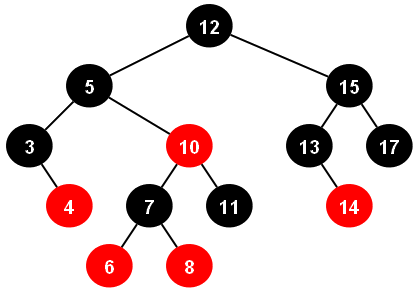
\includegraphics[width=0.45\textwidth]{pictures/redblacktree.png}
%	\caption{RED-BLACK-TREE~\protect\cite{rtoal}}
	\caption{Rot-Schwarz-Baum}
	\label{fig:rbtree}
\end{figure}

 
Nach \cite{tcormen} müssen folgende Regeln eingehalten werden, damit ein Rot-Schwarz-Baum zustande kommt:

\begin{enumerate}
	\item Jeder Knoten ist entweder rot oder schwarz.
	\item Die Wurzel ist schwarz.
	\item Jedes Blatt (NIL) ist schwarz.
	\item Wenn ein Knoten rot ist, dann sind seine beiden Kinder schwarz.
	\item Für jeden Knoten enthalten alle einfachen Pfade, die an diesem Knoten starten und in einem Blatt des Teilbaumes dieses Knotens enden, die gleiche Anzahl schwarzer Knoten. 
\end{enumerate}

Wie bereits Thomas H. Cormen in \cite{tcormen} beweist, kann ein Baum, welcher nach diesen Regeln erstellt wird, eine maximale Höhe von $2lg(n+1)$ erreichen. Damit ergeben sich die Laufzeiten für verschiedene Operation, wie z.B. das Suchen im Baum, auf einen Maximalwert von $O(lg\, n)$.

Beim Einfügen oder Löschen in den Baum werden Verbindungen oder Knoten verändert. Dabei kann es passieren, dass der Baum wieder in ein Ungleichgewicht gerät. 
Um dieser Problematik entgegen zu wirken, werden spezielle Einfüge- bzw. Lösch\-operationen angewendet, welche so konstruiert sind, dass immer die fünf oben genannten Regeln eingehalten werden. 

So müssen innerhalb dieser Einfüge- oder Lösch\-ope\-ra\-ti\-on\-en z.B. Rotationen von Knoten unter bestimmten Bedingung durchgeführt oder die Farben bzw. auch die Zeigerstruktur geändert werden.

Werden die fünf Regeln unter allen Bedingungen und zu jeder Zeit eingehalten, so kann immer die maximale Laufzeit garantiert werden und außerdem können der kleinste und der größte Schlüssel immer direkt auf der linkesten bzw. auf der rechtesten Seite gefunden werden.
%Mit den Regeln von RED-BLACK wird mit Hilfe von z.B. Rotationen um das den Parent Knoten, immer für das richtige Gleichgewicht gesorgt.

